
%
%
\documentclass{article}
\usepackage{amsmath}
\usepackage{graphicx}
\usepackage{color}
\usepackage{amsfonts}
\usepackage[margin=2.5cm,bmargin=.5cm]{geometry}
%\usepackage{showframe}
\newcommand{\cE}{\mathcal{E}}                               %
\setlength{\voffset}{-2cm}

\begin{document}

\title{Summary of summer project}
\author{Dominic Skinner}
\date{}
\maketitle
\pagenumbering{gobble}
\section*{Introduction}
Consider a semi-infinite elastic solid with a thin strip peeled off, and the
resulting crack filled with an incompressible fluid. The motion is driven
by a bending moment applied to the ``arm'' of the solid. The aim is to be
able to write down a set of equations governing the dynamics, in particular
it is of interest to examine the realationship between the speed of traveling
wave solutions $c$, the magnitude of the bending moment $M$, and the toughness 
of the solid $K_I$. 
\\
\\
Relevant physical problems include the formation of hydrofractures in an oil
reservoir, or of igneous intrusions beneath a volcano, since both involve
the propagation of a crack through a brittle elastic solid driven by fluid 
injection.
\\
\\
This is a joint work with Tim Large, who started this project in
summer 2014.
\section*{Set up}
\begin{minipage}{0.5\linewidth}
We assume that the flow everywhere satisfies the lubrication equations. From 
fluid mechanics, we then get the equation
\[12\mu c = h^2 p'\]
From elasticity, using Muskhelishiveli methods, we can derive the equation
\[
{ p \choose 0 }  =
\frac{E}{4\pi (1-\nu^2)} \int
%\underline{\underline{K}}(x-z) 
\left(\begin{array}{cc} K_{11} & K_{12} \\ K_{21} & K_{22} \end{array} \right)
{ g' \choose h' }  \]
Where $K_{ij}$ is the integral kernel specific to this geometry.
\end{minipage}
\begin{minipage}{0.07\linewidth}
~
\end{minipage}
\begin{minipage}{0.4\linewidth}
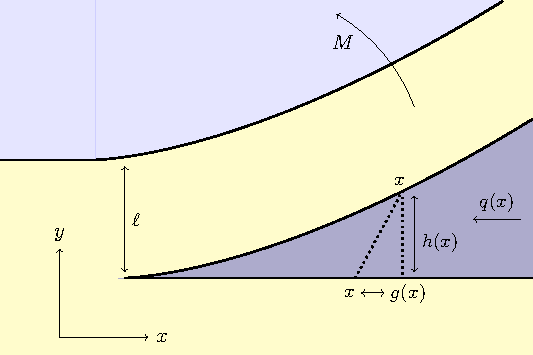
\includegraphics[scale=0.75]{Fig1.pdf}
\end{minipage}
\\
\\
$E$ is the Young's modulus of the solid, $\nu$ is Poisson's ratio, $\mu$ is 
the viscosity of the fluid.
The boundary conditions on the solid at $\infty$ are governed by the bending 
moment, using the beam approximation. The boundary conditions near the crack
tip are governed by ``Linear Elastic Fracture Mechanics''. 

A problem of 
particular interest is the ``Small toughness'' problem, when 
$K_I \ll M \ell^{-3/2}$. The near tip asymptotics when $K_I=0$, namely
$h \sim x^{2/3}$ need to be reconciled with the asymptotics for 
$K_I>0$, where $h \sim x^{1/2}$. The result is a near tip boundary layer.
\section*{Results}
The two equations above (together with boundary condtions) have been solved
numerically. Analytic methods have also been applied; it was found that 
by approaching asymptotically close to the crack tip, the geomety reduces
to a known problem. This allows us to obtain the ``Small toughness'' 
solution
\[ c = \frac{36(1-\nu^2)^2M^3}{\pi \mu E^2 \ell^5}\left(\lambda_0 + C 
\lambda_0^{2s-1}\lambda_1 (\ell^{3/2}K_I/M)^u \right) \]
The constants $\lambda_0$,$\lambda_1$, $C$, $u$,$s$, have been determined 
numerically. This result is in close agreement with numerical solutions.

\end{document}
